
\chapter{Aplicação e Resultados} \label{chap:4}


\section{O Simulador Pipesim}
Sistemas de produção de petróleo são sistemas nos quais se deseja sempre produzir o máximo possível e de forma segura.
O PIPESIM, da Schlumberger, é um simulador de fluxo multifásico em regime permanente que pode ser utilizado tanto para o projeto como para planejamento de operações em campos de petróleo. Ele permite que sejam simuladas situações alternativas de forma mais rápida e segura que testes reais.

\section{Interface}
Para interfaceamento do Pipesim com outros softwares, a Schlumberger disponibiliza uma API chamada OpenLink. Esta pode ser utilizada para interação programática com o Pipesim, habilitando a configuração de novos poços, análise, simulações, e automação da simulação. Utilizando-se a biblioteca pyWin32, é possível comunicar-se com a API, mas apenas no windows de 32 bits.

\section{Experimentos}
Foi realizado um experimento de sintonia de curva, e utilizados três abordagens diferentes para a sintonia. Primeiramente foi utilizado o orthoMADS, com a implementação NOMAD, em seguida, foi utilizado novamente o NOMAD, mas com surrogate model calculado pela SGTELIB, e finalmente, uma implementação do Nelder-Mead Simplex. Os resultados então são comparados quanto a numero de avaliações e acuracia do resultado.

\subsection{O Problema de sintonia}
Primeiramente foi configurado um unico poço de petróleo, que pode ser visto na figura \ref{fig:setup1_dia}. A seguir foram escolhidos dados arbitrariamente para compor a curva "real" de produção (figura \ref{fig:truth1}).
Neste Experimento a curva sintonizada foi a de fluxo de líquido (Barris padrões por dia) por gás injetado (milhões de pés cúbicos padrões por dia). Escolheu-se a pressão estática do reservatório como sendo 4000 psi absoluto, e um indice de produtividade liquido de 25 STDB/d/psi( Barris padrões por dia por pressão estática). Desta forma a figura \ref{fig:truth1} demonstra a curva "real" a ser sintonizada.



\begin{figure}
\centering
\begin{subfigure}{.4\textwidth}
  \centering
  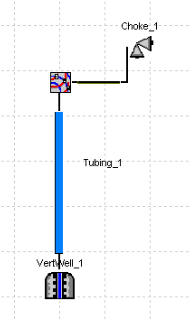
\includegraphics[height=1\linewidth]{figs/setup1.png}
  \caption{Setup do poço de petróleo.}
  \label{fig:setup1_dia}
\end{subfigure}%
\begin{subfigure}{.6\textwidth}
  \centering
  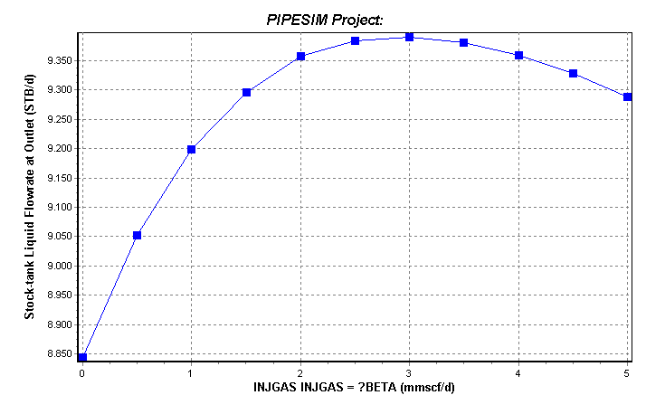
\includegraphics[height=0.7\linewidth]{figs/truth1.png}
  \caption{Curva "real" do poço de petróleo.}
  \label{fig:truth1}
\end{subfigure}
\caption{Experimento 1.}
\label{fig:setup1}
\end{figure}

Para os testes, os parametros SP (pressão estática) e Liq PI (Índice de produção de líquido) foram iniciados respecticamente em 3000 e 15.


\subsection{Sintonia de curva com o orthoMADS}
Para a sintonia com o orthoMADS, foi utilizada o framework OPAL (A Framework for Optimization of Algorithms), interface python para o solver NOMAD.
A implementação com o OPAL utiliza dois arquivos, "well\_declaration.py" e "well\_optimize.py".

O arquivo "well\_declaration.py" expõe os componentes do problema:

\begin{itemize}
\item Nome do algoritmo:
\begin{verbatim}
# Define Algorithm object.
tuning = Algorithm(name='TUNING', description='Well Tuning')
\end{verbatim}
\end{itemize}

\begin{itemize}
\item Comando utilizado pelo solver para avaliar a função:
\begin{verbatim}
tuning.set_executable_command('python pipesim_run.py')
\end{verbatim}
\end{itemize}


\begin{itemize}
\item As variáveis de decisão:
\begin{verbatim}
static_pressure = Parameter(kind='real', 
                            default=sp, 
                            bound=(2000, 7000),
                            name='sp', 
                            description='Static Pressure')
liq_pi = Parameter(kind='real', 
                   default=pi, 
                   bound=(15, 35),
                   name='pi', 
                   description='Liq PI')

FD.add_param(static_pressure)
FD.add_param(liq_pi)
\end{verbatim}
\end{itemize}

\begin{itemize}
\item E o erro:
\begin{verbatim}
error = Measure(kind='real', name='ERROR', description='Curve quadratic error')
FD.add_measure(error)
\end{verbatim}
\end{itemize}

Já no arquivo "well\_optimize", são declarados

Adicionalmente, foi importo o seguinte solver do NOMAD:
\begin{align}
F\_TARGET = 0.1
\end{align}
De modo a limitar o tamanho mínimo da malha, e terminar a simulação quando o erro ficar menor que $10^{-5}$

em 467 segundos (7:47 minutos) o noMADS convergiu para SP=4004.15, PI = 24.72, com a função custo em 0.896. A parada se deu pelo MIN\_MESH\_SIZE. A performance do algoritmo pode ser vista na figura \ref{fig:setup1_points}


\begin{figure}
\centering
\begin{subfigure}{0.5\textwidth}
  \centering
  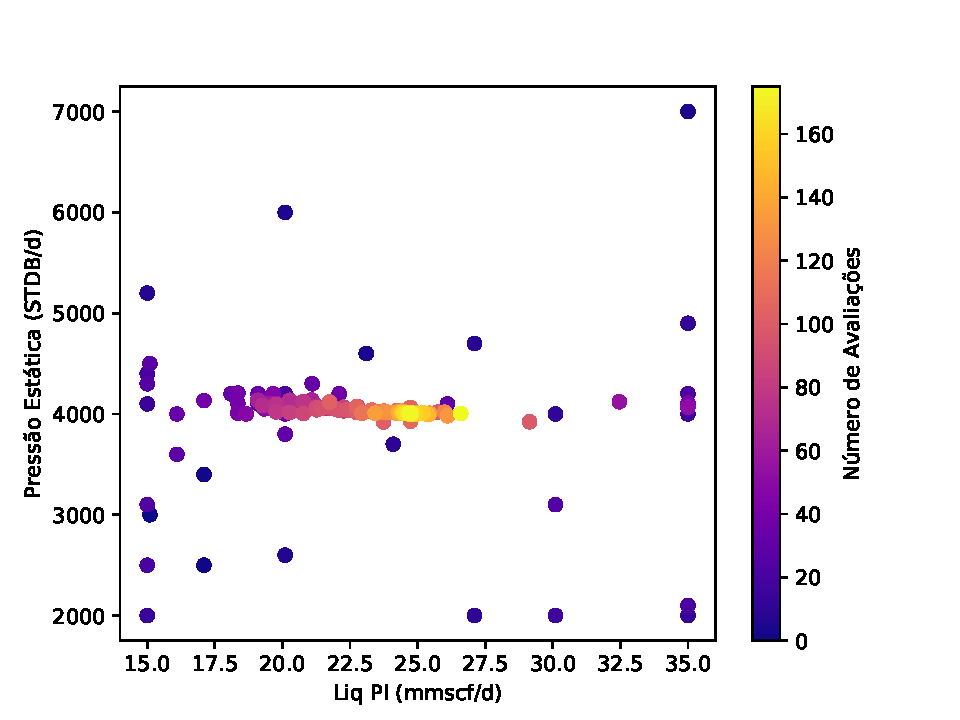
\includegraphics[width=1\linewidth]{figs/setup1_eval_points.pdf}
  \caption{Pontos escolhidos pelo noMADS.}
  \label{fig:setup1_points}
\end{subfigure}%
\begin{subfigure}{0.5\textwidth}
  \centering
  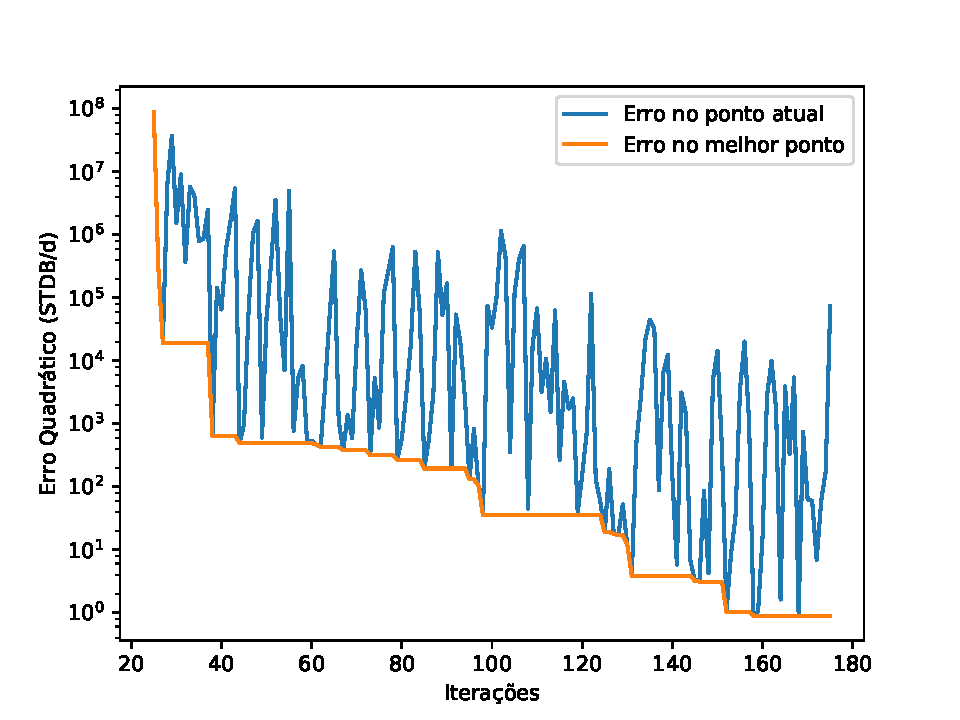
\includegraphics[width=1\linewidth]{figs/setup1_errors.pdf}
  \caption{Erro nos pontos avaliados.}
  \label{fig:setup1_error}
\end{subfigure}
\caption{Experimento 1.}
\label{fig:setup1_2}
\end{figure}

\subsection{Surrogate Lib}

Durante a realização desses experimentos, o noMAD foi atualizado e recebeu uma ferramenta auxiliar, uma biblioteca que tenta aproximar a função a partir dos pontos já utilizados, para utilização no passo "search" do algoritmo. Esta biblioteca faz com que o algoritmo, a cada iteração, tente adivinhar a melhor direção para avançar, ao invés de progredir aleatoriamente.



\section{Discussion}





%%%%%%%%%%%%%%%
